\section{Resultados}

Para os todos métodos, variou-se os parâmetros a fim de encontrar os melhores desempenhos, tanto em tempo quanto em acurácia. Para os resultados apresentados a seguir, utilizou-se os parâmetros mencionados na Seção \ref{sec:metodologia}. Apresentam-se a seguir os resultados obtidos para cada partição em cada uma dos métodos, assim como as respectivas curvas de aprendizado.

\subsection{KNN}

Visando obter as melhores acurácias e tempos de treinamento, selecionou-se o valor K = 51, obtendo-se os resultados apresentados na Tabela \ref{table:resultadosKNN}. A curva de aprendizado para este método não pode ser obtida dada a complexidade computacional.

\begin{table}[h]
\centering
\caption{Resultados para o KNN sendo K = 51}
\vspace{0.2cm}
\begin{tabular}{c|c|c|c|c|c}
Partição & Acurácia & F-medida & Precisão & Revocação & Tempo \\
\hline
1  & 0,74607 & 0,74607 & 0,74607 & 0,74607 & 37,549 \\
2  & 0,75515 & 0,75515 & 0,75515 & 0,75515 & 37,233 \\
3  & 0,74925 & 0,74925 & 0,74925 & 0,74925 & 37,347 \\
4  & 0,75603 & 0,75603 & 0,75603 & 0,75603 & 38,548 \\
5  & 0,76179 & 0,76179 & 0,76179 & 0,76179 & 39,026 \\
6  & 0,74662 & 0,74662 & 0,74662 & 0,74662 & 38,081 \\
7  & 0,75293 & 0,75293 & 0,75293 & 0,75293 & 37,536 \\
8  & 0,75183 & 0,75183 & 0,75183 & 0,75183 & 36,817 \\
9  & 0,75803 & 0,75803 & 0,75803 & 0,75803 & 36,604 \\
10 & 0,74341 & 0,74341 & 0,74341 & 0,74341 & 36,824 \\
\hline
Média & 0,75211 & 0,75211 & 0,75211 & 0,75211 & 37,557

\end{tabular} 
\label{table:resultadosKNN}
\end{table}

\subsection{Regressão logística}

Para efetuar a vizualização do comportamento do método, criou-se o gráfico mostrando a curva de aprendizagem, como se pode observar na Figura \ref{fig:RL}.

\begin{figure}[h]
\centering
\makebox[\columnwidth]{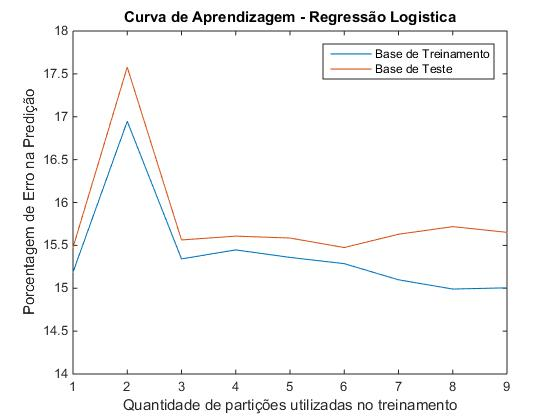
\includegraphics[width=\columnwidth]{RL}}
\caption{Curva de Aprendizagem - Regressão Logistica}
\label{fig:RL}
\end{figure}

Observou-se que o método não está sofrendo de superajustamento, dado que as curvas estão próximas. E não está sofrendo de subajustamento, pois o erro está baixo, dessa forma o método se mostra estável e com um bom ajuste.

Visando obter-se as melhores acurácias e tempos de treinamento, selecionou-se a hipótese linear com um fator de regularização \(\lambda\) = 100, obtendo-se os resultados apresentados na Tabela \ref{table:resultadosRL}.

\begin{table}[h]
\centering
\caption{Resultados para a Regressão Logística sendo a hipótese linear e \(\lambda\) = 100}
\vspace{0.2cm}
\begin{tabular}{c|c|c|c|c|c}
Partição & Acurácia & F-medida & Precisão & Revocação & Tempo \\
\hline
1  & 0,86062 & 0,85909 & 0,86581 & 0,85754 & 56,846 \\      
2  & 0,86322 & 0,86180 & 0,86875 & 0,86040 & 30,724 \\      
3  & 0,85977 & 0,85811 & 0,86674 & 0,85663 & 54,428 \\      
4  & 0,86047 & 0,85899 & 0,86679 & 0,85769 & 43,907 \\      
5  & 0,86992 & 0,86865 & 0,87501 & 0,86724 & 43,519 \\      
6  & 0,86648 & 0,86497 & 0,87144 & 0,86328 & 33,003 \\      
7  & 0,86945 & 0,86790 & 0,87574 & 0,86622 & 51,874 \\    
8  & 0,86793 & 0,86640 & 0,87390 & 0,86475 & 41,304 \\      
9  & 0,86943 & 0,86804 & 0,87503 & 0,86652 & 43,230 \\      
10 & 0,86492 & 0,86317 & 0,87150 & 0,86134 & 30,503 \\
\hline
Média & 0,86522 & 0,86371 & 0,87107 & 0,86216 & 42,934

\end{tabular} 
\label{table:resultadosRL}
\end{table}

\subsection{Redes Neurais Artificiais}
	
Para efetuar a vizualização do comportamento do método, criou-se o gráfico mostrando a curva de aprendizagem como se pode observar na Figura \ref{fig:RNA}.

\begin{figure}[h]
\centering
\makebox[\columnwidth]{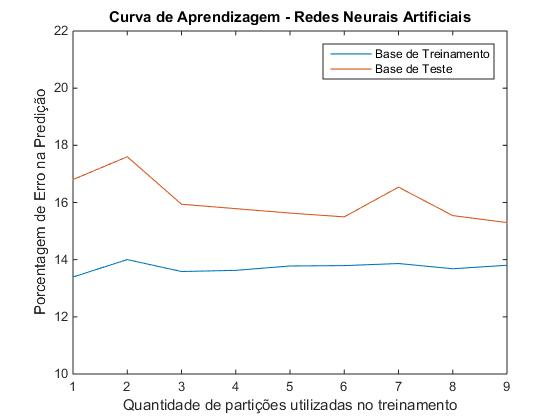
\includegraphics[width=\columnwidth]{RNA}}
\caption{Curva de Aprendizagem - Redes Neurais Artificiais}
\label{fig:RNA}
\end{figure}

Observou-se que o método não está sofrendo de superajustamento dado que as curvas estão próximas, e não esta sofrendo de subajustamento, pois o erro está baixo, dessa forma o método se demonstra estável e com um bom ajuste. Também é possível observar que já no começo do ajuste os dados já estavam com um bom resultado, e aumentar a base não gerou melhora significativa.

Visando obter as melhores acurácias e tempos de treinamento, selecionou-se como taxa de aprendizagem \(\alpha\) = 0,06 e quantidade de neurônios na camada intermediária com 50 elementos, obtendo-se os resultados apresentados na Tabela \ref{table:resultadosRNA}.

\begin{table}[h]
\centering
\caption{Resultados para RNA}
\vspace{0.2cm}
\begin{tabular}{c|c|c|c|c|c}
Partição & Acurácia & F-medida & Precisão & Revocação & Tempo \\
\hline
1  & 0.87130 & 0.87011 & 0.87348 & 0.86872 & 94,369 \\
2  & 0.87854 & 0.87746 & 0.88080 & 0.87608 & 102,94 \\
3  & 0.87930 & 0.87805 & 0.88231 & 0.87640 & 119,73 \\
4  & 0.87350 & 0.87238 & 0.87633 & 0.87098 & 90,938 \\
5  & 0.87731 & 0.87635 & 0.87938 & 0.87513 & 101,33 \\
6  & 0.87793 & 0.87677 & 0.87986 & 0.87535 & 105,95 \\
7  & 0.88325 & 0.88209 & 0.88588 & 0.88052 & 129,29 \\
8  & 0.86936 & 0.86822 & 0.87192 & 0.86687 & 148,67 \\
9  & 0.88188 & 0.88083 & 0.88421 & 0.87942 & 119,64 \\
10 & 0.87991 & 0.87862 & 0.88239 & 0.87697 & 113,08 \\
\hline
Média & 0.87723 & 0.87609 & 0.87966 & 0.87464 & 112,59 \\
\end{tabular} 
\label{table:resultadosRNA}
\end{table}

\subsection{Máquinas de vetores de suporte}
	
Para efetuar a vizualização do comportamento do método, criou-se o gráfico mostrando a curva de aprendizagem como se pode observar na Figura \ref{fig:SVM}.

\begin{figure}[h]
	\centering
\makebox[\columnwidth]{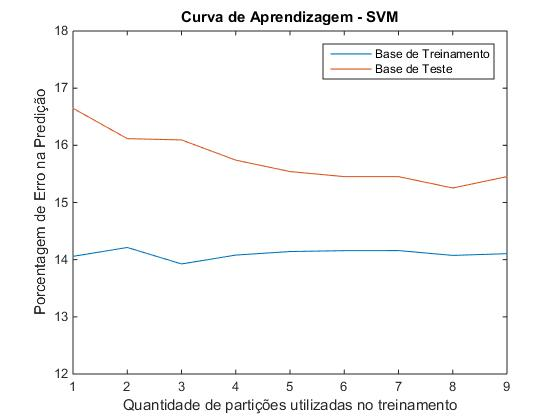
\includegraphics[width=\columnwidth]{SVM}}
\caption{Curva de Aprendizagem - SVM}
\label{fig:SVM}
\end{figure}

Observou-se que o método não está sofrendo de superajustamento dado que as curvas estão próximas, e não esta sofrendo de subajustamento, pois o erro está baixo, dessa forma o método se mostra estável e com um bom ajuste. 

Visando obter as melhores acurácias e tempos de treinamento, selecionou-se duas opções para o SVM, uma com kernel linear e parâmetro de custo \emph{C} = 0.01, apresentando-se os resultados na Tabela \ref{table:resultadosSVMLinear} e uma com kernel radial, parâmetros de custo \emph{C} = 1 e parâmetro \(\gamma\) = 0.01, apresentando os resultados na Tabela \ref{table:resultadosSVMRadial}

\begin{table}[h]
\centering
\caption{Resultados para SVM com kernel linear e C = 0.01}
\vspace{0.2cm}
\begin{tabular}{c|c|c|c|c|c}
Partição & Acurácia & F-medida & Precisão & Revocação & Tempo \\
\hline
1  & 0,84725 & 0,84635 & 0,84835 & 0,84553 & 387,15 \\ 
2  & 0,85753 & 0,85665 & 0,85894 & 0,85575 & 371,86 \\
3  & 0,85985 & 0,85886 & 0,86134 & 0,85784 & 398,54 \\
4  & 0,85467 & 0,85379 & 0,85627 & 0,85291 & 396,04 \\
5  & 0,86017 & 0,85941 & 0,86129 & 0,85862 & 370,89 \\
6  & 0,85363 & 0,85271 & 0,85463 & 0,85186 & 371,20 \\
7  & 0,86295 & 0,86198 & 0,86457 & 0,86094 & 371,87 \\
8  & 0,86137 & 0,86044 & 0,86265 & 0,85948 & 373,39 \\
9  & 0,85854 & 0,85770 & 0,85991 & 0,85684 & 371,56 \\
10 & 0,85725 & 0,85617 & 0,85880 & 0,85508 & 371,22 \\
\hline
Média & 0,85732 & 0,85641 & 0,85867 & 0,85548 & 378,37 \\

\end{tabular} 
\label{table:resultadosSVMLinear}
\end{table}

\begin{table}[h]
\centering
\caption{Resultados para SVM com kernel radial, C = 1 e \(\gamma\) = 0.01}
\vspace{0.2cm}
\begin{tabular}{c|c|c|c|c|c}
Partição & Acurácia & F-medida & Precisão & Revocação & Tempo \\
\hline
1  & 0,84725 & 0,84635 & 0,84835 & 0,84553 & 387,15 \\ 
2  & 0,85753 & 0,85665 & 0,85894 & 0,85575 & 371,86 \\
3  & 0,85985 & 0,85886 & 0,86134 & 0,85784 & 398,54 \\
4  & 0,85467 & 0,85379 & 0,85627 & 0,85291 & 396,04 \\
5  & 0,86017 & 0,85941 & 0,86129 & 0,85862 & 370,89 \\
6  & 0,85363 & 0,85271 & 0,85463 & 0,85186 & 371,20 \\
7  & 0,86295 & 0,86198 & 0,86457 & 0,86094 & 371,87 \\
8  & 0,86137 & 0,86044 & 0,86265 & 0,85948 & 373,39 \\
9  & 0,85854 & 0,85770 & 0,85991 & 0,85684 & 371,56 \\
10 & 0,85725 & 0,85617 & 0,85880 & 0,85508 & 371,22 \\
\hline
Média & 0,85732 & 0,85641 & 0,85867 & 0,85548 & 378,37 \\

\end{tabular} 
\label{table:resultadosSVMRadial}
\end{table}

\subsection{Naive Bayes}
	
Para efetuar a vizualização do comportamento do método, criou-se o gráfico mostrando a curva de aprendizagem como pode-se observar na Figura \ref{fig:NaiveBayes}.

\begin{figure}[h]
	\centering
\makebox[\columnwidth]{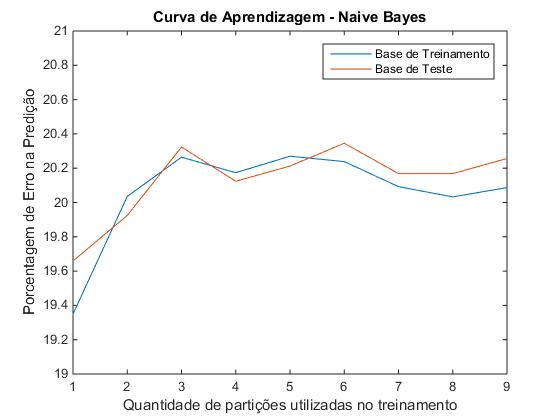
\includegraphics[width=\columnwidth]{NaiveBayes}}
\caption{Curva de Aprendizagem - Naive Bayes}
\label{fig:NaiveBayes}
\end{figure}

Observou-se que o método não está sofrendo de superajustamento, dado que as curvas estão próximas, e não está sofrendo de subajustamento, pois o erro está baixo. Dessa forma o método se mostra estável e com um bom ajuste.

\begin{table}[h]
\centering
\caption{Resultados para Naive Bayes}
\vspace{0.2cm}
\begin{tabular}{c|c|c|c|c|c}
Partição & Acurácia & F-medida & Precisão & Revocação & Tempo \\
\hline
1  & 0,84255 & 0,84031 & 0,85452 & 0,83972 & 1,5254 \\
2  & 0,84731 & 0,84506 & 0,86158 & 0,84486 & 1,5465 \\
3  & 0,84693 & 0,84463 & 0,86029 & 0,84408 & 1,5446 \\
4  & 0,84498 & 0,84278 & 0,85891 & 0,84272 & 1,5119 \\
5  & 0,84862 & 0,84670 & 0,86086 & 0,84650 & 1,5206 \\
6  & 0,84920 & 0,84690 & 0,86174 & 0,84603 & 1,5198 \\
7  & 0,84499 & 0,84272 & 0,85898 & 0,84251 & 1,5126 \\
8  & 0,85428 & 0,85205 & 0,86754 & 0,85119 & 1,5395 \\
9  & 0,85367 & 0,85163 & 0,86632 & 0,85104 & 1,5342 \\
10 & 0,84597 & 0,84349 & 0,85954 & 0,84274 & 1,5229 \\
\hline
Média & 0,84785 & 0,84563 & 0,86103 & 0,84514 & 1,5278 \\

\end{tabular} 
\label{table:resultadosNB}
\end{table}

\section{Resultados gerais}

O comparativo geral entre os métodos é apresentado na Tabela \ref{table:resultadosGerais} pela média das execuções dos métodos, os melhores resultados para cada parâmetros estão destacados em negrito.

\begin{table}[h]
\centering
\caption{Resultados gerais}
\vspace{0.2cm}
\begin{tabular}{c|c|c|c|c|c}
Método & Acurácia & F-medida & Precisão & Revocação & Tempo \\
\hline
KNN                & 0,75211 & 0,75211 & 0,75211 & 0,75211 & 37,557 \\
Regresão Log.      & 0,86522 & 0,86371 & 0,87107 & 0,86216 & 42,934 \\
RNA                & \textbf{0.87723} & \textbf{0.87609} & \textbf{0.87966} & \textbf{0.87464} & 112,59 \\
SVM Linear         & 0,85732 & 0,85641 & 0,85867 & 0,85548 & 378,37 \\
SVM Radial         & 0,85732 & 0,85641 & 0,85867 & 0,85548 & 378,37 \\
Naive Bayes        & 0,84785 & 0,84563 & 0,86103 & 0,84514 & \textbf{1,5278} \\
\end{tabular}
\label{table:resultadosGerais}
\end{table}


